\documentclass[conference]{IEEEtran}
% The preceding line is only needed to identify funding in the first footnote. If that is unneeded, please comment it out.
\usepackage{cite}
\usepackage{amsmath,amssymb,amsfonts}
\usepackage{algorithmic}
\usepackage{graphicx}
\usepackage{textcomp}
\usepackage{xcolor}
\def\BibTeX{{\rm B\kern-.05em{\sc i\kern-.025em b}\kern-.08em
    T\kern-.1667em\lower.7ex\hbox{E}\kern-.125emX}}
\begin{document}

\title{Summary of “An Investigation into Android In-App Ad Practice: Implications for App Developers”  \\
}

\author{\IEEEauthorblockN{Stephane Meunier}
\IEEEauthorblockA{\textit{Department of Mathematics and Computer Science} \\
\textit{Clark University}\\
Worcester, Massachusetts \\
smeunier@clarku.edu}
\and
\IEEEauthorblockN{Catalin Veghes}
\IEEEauthorblockA{\textit{Department of Mathematics and Computer Science} \\
\textit{Clark University}\\
Worcester, Massachusetts \\
cveghes@clarku.edu}
}

\maketitle

\begin{abstract}
The purpose of this paper is to summarize the work\cite{ReferencePaper} conducted by Boyuan He, Haitao Xu, Ling Jin, Guanyu Guo, Yan Chen, and Guangyao Weng during their research which was published in IEEE INFOCOM 2018 Conference.

In-app advertising represents the major source of income for millions of developers and application owners. To monetize their mobile apps, these people commonly utilize various ad networks and ad types to generate revenues in order to sustain their products. Even though it is a widespread habit, especially among free applications which do not charge users for downloading the software, there are neither formal studies nor recommendations about this segment’s best practices. The conference paper under discussion strives to reveal suitable implementations for advertisements and provide stakeholders guidelines on ad network selection and ad placement to maximize income without affecting the overall user experience. While working on this paper, the authors investigated 277,616 Android apps and extracted 697 unique APIs belonging to 164 ad networks. Based on the similarities they observed between different advertisements, the team was able to classify them into five ad types: Embedded, Popup, Notification, Offerwall, and Floating. These are the basic categories which are being used throughout the research in order to concisely articulate their findings among a significant number of alike yet different kinds of advertisements.
\end{abstract}

\begin{IEEEkeywords}
in-app ads, Android, mobile applications, API, advertisements, ad networks.
\end{IEEEkeywords}

\section{Introduction}
\subsection{Motivation and State of the Art}
The focus of this work is the Android platform which has increasingly become the dominant operating system for mobile devices. Its salient importance is supported by numbers and facts rigorously cited and examined by the authors. Android’s worldwide market share has hit 86.1\% in the first quarter of 2017 and the number of apps in Google Play has reached 2.9 million in the February 2017, 95\% of which are free apps\cite{Gartner}. As most of the free apps leverage third-party in-app advertising for generating money, having a good understanding of ad networks and their associated ad types is of great importance. According to an economic forecast\cite{Visionmobile}, the in-app advertising market is worth around 62 billion US dollars and significantly affects thousands of people at an economic level. Therefore, by providing clear rules and principles, this research is extremely valuable as in-depth analysis and coherent guidelines are essential for adequate development of the in-app advertisement segment. Although the mobile advertising ecosystem has been the subject of numerous recent researches, most of the efforts focus on security, the privacy of ad networks, mobile ad fraud, and ad targeting. The current state of the art does not include any published materials that address the challenge tackled in this paper.

\subsection{Contribution}
To provide a reliable set of principles to follow when it comes to choosing best ad networks and appropriate ad types, the paper studies Android in-app advertising from a developer’s perspective. The authors developed a static analysis framework for Android apps called MAdLens. MAdLens was used to automate the tedious task of extracting relevant information from the pool of 277,616 free Android applications, randomly selected from Google Play Store. Leveraging on this system, they further performed a large-scale measurement across the Android market and identified trends in the usage of mobile ad networks, aggressiveness difference of ad types and its impact on the usability of the apps. There are three major contributions made by this research:
\begin{itemize}
\item It is the first to provide practical guidelines for stakeholders to monetize their apps through third-party in-app advertising.
\item It is the first to map APIs of ad networks to specific ad types and measure third-party in-app advertising in Android apps at API granularity.
\item It is the first to provide a unified classification system for mobile in-app ads and measure the impact of different ad types on apps.
\end{itemize}

\subsection{Paper Structure}
The first Section of their paper includes the abstract and the introduction which present the issue, its significance in the contemporary context, the concepts behind MAdLens, and some notable findings of in-app mobile advertising. Section 2 provides relevant background in Android third-party ads, while Section 3 offers a detailed analysis of MAdLens system as well as a comprehensive discussion of the methodology used by this system. Section 4 demonstrates the result of their large-scale measurements and gives explanations as well as implications based on their results. Section 5 discusses the limitations of their work. Section 6 presents related work and Section 7 concludes the paper.

\section{Related Works}
In recent years, mobile advertising has become an important topic for research especially because of the security concerns that it poses. Some of the preeminent materials mentioned in this paper study topics like the potential risks of embedded or in-app ad libraries \cite{Grace}, the risk associated with user data exposure to advertising libraries \cite{meng2016price}, a privacy protection framework to “achieve an equilibrium” between the developer’s revenue and the user’s privacy \cite{leontiadis2012don}, the mobile ad fraud perpetrated by Android apps \cite{crussell2014madfraud}, the user targeting strategies of top ad networks \cite{nath2015madscope}, or the use of machine-learning to detect ad libraries and then use code instrumentation to deescalate their unnecessary privileges \cite{liu2015efficient}.
All these materials inspect the amount of sensitive information and the ways ad libraries handle it in order to provide relevant ads to the end users while preserving their individual privacy. For example, one of the studies showed that most existing libraries collect private information for legitimate targeting purposes (such as the user’s location) along with additional data whose purpose is hard to justify (such as the user’s call logs, phone number, browser bookmarks, or even the list of apps installed on the phone). Moreover, some libraries make use of an unsafe mechanism to directly fetch and run code from the Internet, which immediately leads to serious security risks \cite{Grace}. 
Even though the issue regarding data security and its integrity in mobile applications is often addressed in academic literature, there is no guideline that helps stakeholders to make decisions about the appropriate ads for their software, besides the existing security recommendations. Therefore, the paper under discussion represents the state of the art in its area.

\section{System Model}
\subsection{Mobile Ad Network and its Integration in Apps}
The current ecosystem of mobile advertising involves three major members: the publishers who own a mobile application and who desire to display ads in their software to make revenue, the advertisers who pay to get their content advertised, and the ad networks which serve as intermediate platforms that bridge the connection between the first two members. To integrate the ad network mechanism developers must include one or more pre-compiled ad libraries provided by ad network companies. These libraries and their necessary dependencies are generally implemented in Java and come in the form of compiled jar files. After importing the libraries, programmers can interact with them using specific APIs. Most ad networks provide a rich API surface which allows developers to customize the visual aspects of the ads they are displaying. Additionally, relevant stakeholders need to create an account on the ad network’s website to set up the payment credentials and individual preferences (suitable ad contents, desired ad frequency, layout, format, and others). 

\subsection{Mobile Ad Classification and Aggressiveness}
Advertisements within mobile applications can be displayed in many different forms. The Conference Paper labels each Ad type by their Aggressiveness and their Format. The aggressiveness of any type of mobile ad is defined by how invasive and unpleasant to the user it is. For the types that can be ignored, skipped or closed, the article labels their aggressiveness as being “Low”. On the other hand for those that are more invasive, their aggressiveness falls into the “High” category. According to the piece of writing, Ad Networks support many different ad formats and the ability to decide whichever configuration would suit the best is a quality that any Mobile Developer should possess. After carefully analyzing distinct Ad Networks and their different formats, the authors have decided that classifying the Ads would be the most convenient option. The Research paper categorizes mobile ad in 5 main different types: Offerwall, Popup, Notification, Floating ,and lastly, Embedded.
To begin with, Offerwall is the class of ad that is considered to be one of the most invasive. That is why his aggressiveness is considered to be High. Offerwall uses a reappearing page that offers the client in-app rewards in exchange for completing determined actions (i.e. downloading other apps or watching videos). It often interrupts app’s behavior and cannot be ignored, skip or closed, reason why is considered aggressive. 
Secondly, Notification displays its ad contents the same way that a regular app would display a notification on the mobile device. The main difference between this ad format and the others is that it will still be running even when the app is closed. The advantage for the ad networks of this type is that the notification will be displayed using the same ringtone than other apps tricking the user to look at the mobile device. On the other hand, the disadvantage is that it can distract the user or even interrupt the use of other apps. That is why Notification type is consider to have a High Aggressiveness.
Not all the Ad types are invasive to the user, the research paper categorizes the following 3 Ad type to have Low Aggressiveness.
As its name suggests, Popup type displays a pop-up window in front of the app’s GUI. Popups can take the form of many different sizes and they can even take up the full screen if necessary. Although this type of Ad format could be unpleasant to the user, the research paper categorizes its Aggressiveness as Low. Even though Popups may be invasive and interrupt the app’s behaviour, they can be easily closed by the user. 
Although the Floating type of ad is not very common, it is relevant to the study of different Ad Formats. This category of ad appear in front of GUI of the app with a floating window (why its name). Since it does not often occupy a large portion of the screen, and also can be skipped or closed, the Article categorizes its Aggressiveness as Low. 
Last but not least, the Embedded type of Ad is considered to be the least aggressive format among the others. This Ad Type embeds advertisement content into a small window of the app. It can be displayed in many different ways, such as banner, video and etc. The ads displayed this way usually are very small and do not interrupt the flow of the app. They can also be ignored, skipped or closed.


\section{Methodology}
\begin{figure}[htbp]
	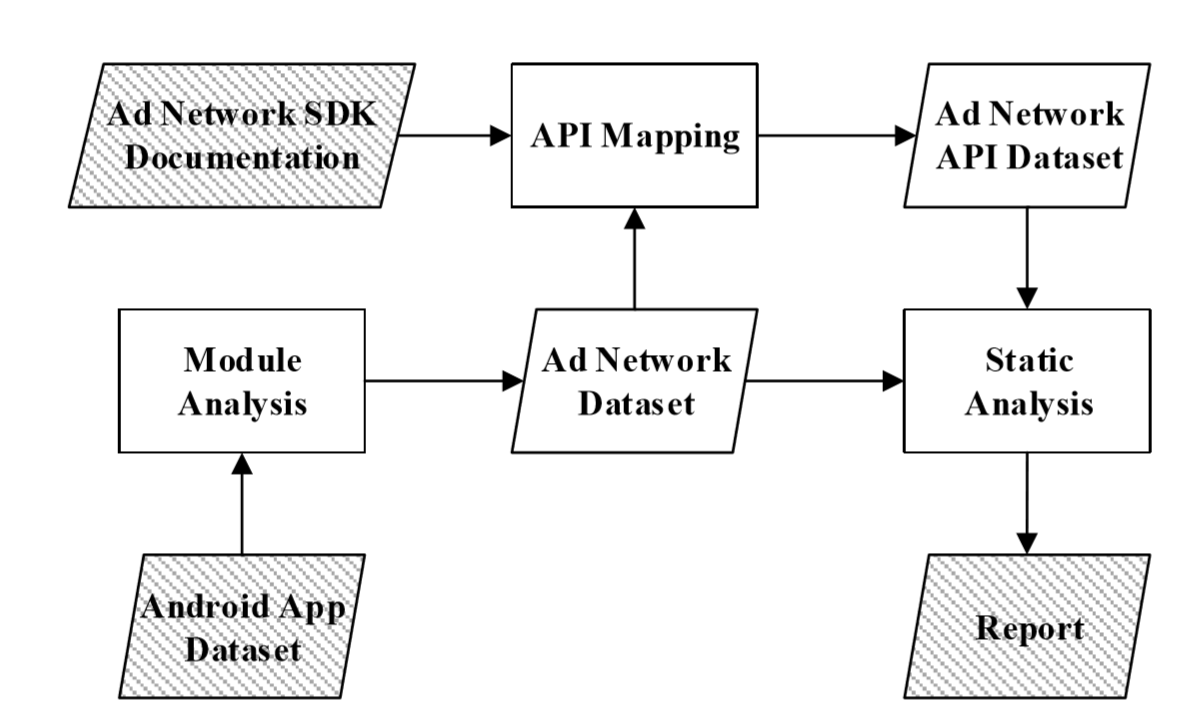
\includegraphics[width=0.5\textwidth,height=0.5\textheight,keepaspectratio]{system.png}
	\caption{Overview of MAdLens}
	\label{fig:system}
\end{figure}
The authors created MAdLens system (Fig. \ref{fig:system} ) which can identify internal third-party ad network modules from an Android app, map APIs of ad networks to specific ad types, and generate a detailed report of all the ad information for each app using static analysis techniques. Part of this system is a crawler that randomly picks applications from Google Play to create the Android App Dataset. For each application in the dataset, MAdLens automatically distinguishes all existing ad networks and then, using the API Mapping created based on Ad network SDK Documentation, classifies the present APIs in one of the five categories defined by the authors and generates an appropriate summary. To extract the relevant information from the applications, the system considers the fact that ads can be implemented either in the resource file (XML) or in Java code. For resources files, they decompile the apk file with Androidguard to get all the Android layout files, then parse all the XML to find the ads. Similarly, for Java code, the smali code is generated by Androguard after decompiling the apk file and ads are recognized in the smali text.

\section{Data Analysis and Results}
The research paper revealed multiple useful discoveries regarding mobile ads for Android applications. Developers may want to pay attention to the different implications that the authors have concluded after conducting a large-scale measurement study. There are 8 crucial implications which arose during the analysis:
\begin{itemize}
\item Due to the rise of different ad networks, developers have many different choices when it comes to determine ad placement in their apps. However, most developers take a more conservative approach when it comes to ads: 71\% of apps contain at most one ad library.
\item When it comes to choosing Ad types, programmers tend to choose Low-Aggressive ad types: Embedded and Popup. They are present in more than half of the analyzed apps. In contrast, the most aggressive types of Ads, Offerwall and Notification, are the least used ad types.
\item The number of Ads in an app is directly correlated with the type of category that app belongs to. The research paper affirms that business or utility apps are much less likely to have ads compared to apps that fall into the category of entertainment or casual.
\item According to the percentage of apps accommodating at least three types of ads, the research paper concludes that the two slightly aggressive ad types, Embedded and Popup, are the most popular among all the different categories. Although Offerwall is the most aggressive type of ad, it is relatively popular. The paper suggests that developers should consider using these three main ad types in their apps to increase their profits.
\item When determining how many different ad libraries to implement in an Android app, a developer should avoid including too many. According to the statistics provided by this research, empirically no more than 6 ad Networks should be added into an app to avoid bad ratings.
\item Developers should take into account the different stages of the app's life cycles when deciding how many ad networks to implement in their apps. When the app is at its initial stage, developers should use at most one ad network. They should use more when the app becomes more popular.
\item The authors propose that developers should opt to mainly use Embedded and Popup ads during any stage of the app's life cycle. Aggressive ad types should be used when their application becomes more mature.
\item Even though the previous implications may suggest that developers should stick to Low-Aggressiveness ads, after analyzing the Aggressiveness of the ads hosted by various applications, the research paper concludes a different idea. Developers can use both Low and High Aggressiveness ads at the same time to maximize their revenue. However, this practice should be carefully implemented and thoughtfully monitored.
\end{itemize}
\section{Limitations and Future Work}
MAdLens takes the static approach of analyzing and extracting the APIs from Android applications. Therefore, it has the inherited limitations of static analysis. The system counts the number of occurrences of various APIs at a specific time and because of the code control flow, some portions of the code are not necessarily executed. Thus, investigated apps could have had additional ads which were not captured by the system because they were not displayed when the experiment was conducted. There are dynamic approaches which can inspect an app’s run-time behavior, but these are still very challenging to implement at a large scale. A viable alternative proposed in the paper was a dynamic solution based on image recognition techniques to identify ad activities on the user interface. However, this option was left by the authors for future work as it required significant additional research.

\section{Conclusion}
The analyzed paper represents one major step forward for the in-app advertising industry. It manages to fill in a gap caused by the lack of theoretical knowledge by providing insights for developers about how to optimize their app monetization with optimal ad placement choices. The authors collected 277,616 Android apps belonging to more than 48 categories and performed a comprehensive exploration before coming up with valuable results. These findings are be able guide any mobile app programmer into Android in-app ad best practice.



\bibliography{ref}
\bibliographystyle{IEEEtran}



\end{document}
